\chapter{Guide for New Users}

\newcommand{\netcdf}{NetCDF}

%%%%%%%%%%%%%%%%%%%%%%%%%%%%%%%%%%%%%%%%%%%%%%%
% Progression Bar
% |==============>   |
% empty chapter        chapter finished
%%%%%%%%%%%%%%%%%%%%%%%%%%%%%%%%%%%%%%%%%%%%%%%

This tutorial is meant for people with some knowledge and/or experience in modelling and Linux, but which have no experience with the ICON model. In the following we will describe in short how to compile and run ICON on your machine. 

\section{Needed Software}

For some components ICON uses external libraries. Therefore you will need some additional software which should be installed on your machine. The following software needed to be installed on your machine:

\begin{itemize}
 \item \netcdf : \netcdf is a set of software libraries and self-describing, machine-independent data formats that support the creation, access, and sharing of array-oriented scientific data.\newline
 (Source: \href{http://www.unidata.ucar.edu/software/netcdf/}{http://www.unidata.ucar.edu/software/netcdf/})
 \item GRIB: GRIB (GRIdded Binary) is a format defined by the WMO (World Meteorological Organization). The use of GRIB in ICON is optional. The ECMWF GRIB API is an application program interface accessible from C, FORTRAN and Python programs developed for encoding and decoding WMO FM-92 GRIB edition 1 and edition 2 messages. A useful set of command line tools is also provided to give quick access to GRIB messages. ICON requires GRIB2 format. \newline
 (Source: \href{https://software.ecmwf.int/wiki/display/GRIB/Home}{https://software.ecmwf.int/wiki/display/GRIB/Home})
 \item MPI: MPI is a library specification for message-passing, proposed as a standard by a broadly based committee of vendors, implementors, and users.\newline
 (Source: \href{http://www.mcs.anl.gov/research/projects/mpi/}{http://www.mcs.anl.gov/research/projects/mpi/})
 \item OpenMP: Jointly defined by a group of major computer hardware and software vendors, the OpenMP API is a portable, scalable model that gives shared-memory parallel programmers a simple and flexible interface for developing parallel applications on platforms ranging from embedded systems and accelerator devices to multicore systems and shared-memory systems.\newline
 (Source: \href{http://openmp.org/wp/}{http://openmp.org/wp/})
\end{itemize}

\section{The Source Code}
% Filenames and URL needs to be adapted
You can obtain the source code on the website of DKRZ:

\href{https://www.dkrz.de/}{https://www.dkrz.de/}

You can use the following commands to untar the ICON source code:

\begin{verbatim}
tar xfvz icon.tar.gz
\end{verbatim}

This will create a folder \verb+icon-1.0+ inside your current directory. Within the ICON User Guide, this folder will further on be called \verb+$ICONDIR+.

\subsection{Directory structure}

Within \verb+$ICONDIR+, you will find a set of subdirectories. The important subdirectories are described in the following. 

\subsubsection{build}

Within the \verb+$ICONDIR/build+ directory, a subdirectory with the name of your computer architecture is created at compilation. Within this subdirectory, a \verb+bin+ subdirectory containing the binary \verb+control_model+ and several further subdirectories containing the compiled module files are created at compilation. 

\subsubsection{config}

Inside the \verb+$ICONDIR/config+ directory, different machine dependent configuration are stored within the configuration files. You can find a description of how to use and set up such configuration files in chapter \ref{chap:UG_config_compil}.

\subsubsection{data}

Within the \verb+$ICONDIR/data+ directory, you will find divers input datasets. For example, there are the datasets \verb+"rrtmg_lw.nc"+ and \verb+"ECHAM6_CldOptProps.nc"+, which are necessary for the radiation scheme (see sec. \ref{InputReal:Rad}). 

\subsubsection{doc}

Within the \verb+$ICONDIR/doc+ directory, several documentations for ICON are stored. There are according subdirectories for scientific (\verb+$ICONDIR/doc/science+), technical (\verb+$ICONDIR/doc/technical+) and programming style guides (\verb+$ICONDIR/doc/style+).

\subsubsection{externals}

Within the \verb+$ICONDIR/externals+ directory, external libraries for ICON are stored. Currently, it is the mtime library which is used to convert different date time formats.

\subsubsection{include}

Within the \verb+$ICONDIR/include+ directory, interfaces to libraries needed by ICON are stored. Currently, the interface to the CDI library is stored inside this directory. 

\subsubsection{run}

Within the \verb+$ICONDIR/run+ directory, namelist descriptor files as well as the full namelist documentation are stored. The namelist descriptor files can be used to generate runscripts. Further information can be found in \ref{chap:UG_running_model}.

\subsubsection{src}

Within the \verb+$ICONDIR/src+ directory, the source code of ICON including the main program and ICON modules can be found. The modules are ordered in several subdirectories which are described in the following. 

The main program \verb+control_model.f90+ can be found inside the subdirectory \newline \verb+$ICONDIR/src/drivers+. Additionally, this directory contains the modules for a hydrostatic and a nonhydrostatic setup.

The configuration of an ICON run is performed within the modules inside \newline \verb+$ICONDIR/src/configure_model+ and \verb+$ICONDIR/src/namelists+. Modules regarding the configuration of idealized test cases can be found inside \verb+$ICONDIR/src/testcases+.

The dynamics of ICON are inside \verb+$ICONDIR/src/atm_dyn_iconam+ and the physical parameterizations inside \verb+$ICONDIR/src/atm_phy_nwp+. Parameterizations for the interactions with the surface can be found inside \verb+$ICONDIR/src/lnd_phy_nwp+.

Shared infrastructure modules for 3-D and 4-D variables can be found within \newline \verb+$ICONDIR/src/shared+. The according routines for 2-D fields (e.g. external parameters) are stored within \verb+$ICONDIR/src/shr_horizontal+.

Modules handling the parallelization can be found in \newline\verb+$ICONDIR/src/parallel_infrastructure+.

Input and output modules are stored in \verb+$ICONDIR/src/io+.

The modules for the grid generator, as described in chapter \ref{chap:UG_grid_generation} can be found inside \newline \verb+$ICONDIR/src/grid_generator+.

\subsubsection{support}

Within the \verb+$ICONDIR/support+ directory, the CDI library is stored. 

\subsubsection{vertical\_coord\_table}

Inside the \verb+$ICONDIR/vertical_coord_tables+ directory, information files describing the relation between model layer and height are stored.

\section{Configuration and Compilation}
\label{chap:UG_config_compil}

%Configure and Compile

To ease up the compilation a configure-file is provided which should take over the main work. This Autoconf configuration is used to analyze the computer architecture (hardware and software) and set user specified preferences, e.g. the compiler. This preferences are read from \verb+config/mh-<OS>+, where \verb+<OS>+ is the identified operating system. Operating systems are listed in the configure-files in \verb+$ICONDIR/config/+ with the according files \verb+mh-<OS>+. If your machine is not listed you can add a config-file with your own \verb+<OS>+ based on the given \verb+mh-<OS>+ files. If different compilers are available, the \verb+mh-<OS>+ file may contain a case construct to distinguish them. If your \verb+<OS>+ is not recognized but is one of the listed \verb+<OS>+ you can invoke the configure file with the according option \verb+--host=$HOST+. Examples for the DWD CRAY system are given in the boxes.

\subsection{Description of the Configuration Files}

To add a specific compiler or change your compiler flags, you have to enter the \newline \verb+$ICONDIR/config/mh-<OS>+ according to your operating system \verb+<OS>+. For the DWD CRAY, the compiler flags in \verb+mh-linux+ look like the following:

\begin{Verbatim}[frame=single]
CRAY EXAMPLE: Compiler Flags inside mh-linux

    config_compiler=cray
	CC          = cc
    FC          = ftn
    F77         = "$FC"
    FFLAGS      = -v -D__LOOP_EXCHANGE -D__MIXED_PRECISION -Df2cFortran 
-e Z -em -hflex_mp=conservative -hfp1 -hadd_paren -r am -Ktrap=divz,ovf
    CFLAGS      = -I${GRIB_API}/include -v -Df2cFortran 
-DHAVE_CF_INTERFACE -DHAVE_LIBNETCDF -DHAVE_LIBGRIB 
-DHAVE_LIBGRIB_API -O3  -D__SVN_VERSION="${SVNVERSION}"
    F77FLAGS    = "$FFLAGS"
    FCLIBS      = "-v"
    GEN_FLAGS   =
    FDEBUG      = -g -R abc
    OMPFLAG     = -mp
    DEFOPT      = -D
    DEFCOPT     = -D
    MODOPT      = -I
    MODDIR      = 
    ;;
\end{Verbatim}

The \verb+cray)+ in this example gives the name of this specific configuration. It can be addressed by a flag at configuration. For this example, the according command to choose this setting would be \verb+./configure --with-fortran=cray+ (see section \ref{sec:config_compile}). Like this, you can create your own configuration by adding a new compiler.

\verb+CC+, \verb+FC+ and \verb+F77+ are the compiler directives for C-Compiler, FORTRAN2003-Compiler and FORTRAN77-Compiler. The according compiler flags are set via \verb+CFLAGS+, \verb+FFLAGS+ and \verb+F77FLAGS+. The variable to set an OpenMP flag is called \verb+OMPFLAG+. Libraries are set via \verb+FCLIBS+. 

\subsection{Configuring and Compiling the Code} \label{sec:config_compile}

To configure the source code go to \verb+$ICONDIR+ and give:

\begin{small}
 \begin{verbatim}
  ./configure
  ./build_command
  \end{verbatim}
\end{small}

If you want to use another compiler than the default compiler you give:

\begin{small}
  \begin{verbatim}
   ./configure --with-fortran=<compiler>
   ./build_command
  \end{verbatim}
\end{small}

where \verb+<compiler>+ is \verb+{gcc,nag,intel,pgi,cray}+.

\begin{Verbatim}[frame=single]
CRAY EXAMPLE: Configure + Make
./configure --with-fortran=cray}
./build_command
\end{Verbatim}

Note, that CRAY compiler environment (cce) versions 8.2.x do not work with ICON. The CRAY configuration is expanded to the following:

\begin{Verbatim}[frame=single]
CRAY EXAMPLE: Configuration
ftn -I../module -v -D__LOOP_EXCHANGE -D__MIXED_PRECISION -Df2cFortran -e 
Z -em -hflex_mp=conservative -hfp1 -hadd_paren -r am -Ktrap=divz,ovf 
-D__ICON__ <object files> -L/usr/local/pkg/grib_api/1.11.0/CRAY/lib  
-L../lib -lsupport -lgrib_api_f90 -lgrib_api -lmtime $(LAPACK_LIB) 
$(NETCDF_LIB) $(HDF5_LIB) $(SZIP_LIB) $(ZLIB_LIB) $(MPI_LIB) 
$(PROFILE_LIB) $(SCT_LIB)
\end{Verbatim}

ICON is parallelized using MPI and OpenMP. You can control the parallelization to be used by giving:

\begin{small}
  \begin{verbatim}
   ./configure --with-mpi/--without-mpi --with-openmp/--without-openmp
   ./build_command
  \end{verbatim}
\end{small}

By default the options are set to \verb+--with-mpi --without-openmp+. After a successful build, you will find the ICON executable named \verb+control_model+ inside \verb+$ICONDIR/build/<OS>/bin/+. The CRAY Fortran compiler is an exception, as the command includes automatically OpenMP. Therefore, although selecting --without-openmp, OpenMP is used.

If you wish to re-configure ICON it is advisable first to clean the old setup by giving:

\begin{small}
  \begin{verbatim}
   make distclean  
  \end{verbatim}
\end{small}

Some more details on configure options can be found in the help of the configure command:

\begin{small}
 \begin{verbatim}
  ./configure --help
 \end{verbatim}
\end{small}

%\section{Running the Model (Test scripts for \icon)}
\section{Running the model (Test scripts for \icon)}\label{sec_cr20140130rjs_test}

\subsection{Principles of testing
  \icon}\label{sec_cr2014_01_30_rjs_principles} 

The \icon{} developers use the buildbot tool in order to perform
automated tests on selected \icon{} experiments at regular time
intervals. The buildbot tool launches the respective test scripts on
various computer platforms and documents success or failure on a special web
site ({\tt https://buildbot.zmaw.de/icon/}). The automated tests are
performed on the newest model revision as available in the \icon{}
repository. Furthermore, tests can be ``forced'', i.e. started by
hand, at any time specifying a certain experiment and model revision
of any branch of the repository. However, it is impossible to test two
revisions against each other or to test a local revision.
Here, we present new tests for \icon{} into which various experiments
are integrated and which are designed
such that they can either be used in the framework of the buildbot
tool or be started manually without reference to buildbot (e.g.~on
a PC at MPI~Hamburg). The tests are designed to trap certain technical
errors and comprise the following experiments:
\begin{description}
\item[{base test:}] Just a simple base run over a short time period
  for a specific experiment. This run will be called
  simulation~A in the following.
\item[{update test:}] In addition to the model revision to test,
  the so--called ``test
  revision'', a ``reference revision'' can be specified. A short
  simulation~A of the test revision over one hour is 
  performed during which restart files are written. The same
  simulation is performed for the reference revision (simulation
  A'). The ``update 
  test'' is said to be passed if there are no differences in the
  output of simulation A and A' using the ``cdo diff'' command on the
  time steps in the output specified by the user.
\item[{restart test:}] In addition to a base simulation~A, a second
  simulation~B restarts \icon{} at some time after the initial date. 
  The ``restart test'' is
  said to be passed if there are no differences in the output for the
  time steps after the restart between the original and the restarted
  simulation using the ``cdo diff'' command. 
\item[{nproma test:}] The nproma test performs a base simulation~A
  and a
  simulation~C with a different value
  of {\tt nproma}. Instead of {\tt nproma} of simulation~A, a value
  of 17 is used 
  in simulation~C or, if ${\tt nproma}=17$ for simulation~A, ${\tt
    nproma}=19$ is used for simulation C. The nproma test is
  said to be passed if the ``cdo diff'' command does not find
  differences in the output.
\item[{mpi parallel test:}] 
  The mpi parallel test performs a base simulation~A and a simulation~D 
  with a reduced number of
  MPI threads compared to the base simulation~A. If more
  than one threads are used on each node, the number of threads on
  each node is reduced by one. If only one thread is used on each
  node, the number of nodes is reduced by one. If only one process is
  used, no mpi parallel test is performed. The parallel test is said
  to be passed if the ``cdo diff'' 
  command does not find differences between the output files.
\item[{openmp parallel test:}]
  The openmp parallel test performs a base simulation~A and a
  simulation~E with a reduced number of
  openmp threads compared to the base simulation~A.
  If only one openmp thread was used, no openmp test is performed.
  The openmp parallel test is said to be passed if the
  ``cdo diff'' 
  command does not find differences between the output files.
\end{description}

The testing procedure is such that tests can be
combined. Furthermore, the test script can be asked to re--use
existing runs without repeating these runs.

Only the following experiments are included into the test script:
\begin{description}
\item[{\bf atm\_amip\_test:}] Non--hydrostatic AMIP--like simulation but with
  transient solar irradiance using \echam{} physics.
\item[{\bf atm\_icoles\_nested:}] Nonhydrostatic atmosphere only
  simulation with a regional 
  grid refinement.
\item[{\bf atm\_jww\_hs\_test:}] Jablonowski Williamson baroclinic
  wave test for a hydrostatic atmosphere.
\item[{\bf oce\_omip\_0160km:}] Ocean only experiment with a 160km
  resolution.
\end{description}

\subsection{Description of test script}

The test script {\tt icon-dev.checksuite} is located in the {\tt
  run/checksuite.icon-dev} 
directory of \icon{} and uses the following run script of the {\tt
  run} directory for the
experiments: ({\it i}\/) {\tt exp.atm\_amip\_test} for the
AMIP--type experiment {\tt atm\_amip\_test}, ({\it ii}\/) {\tt
  exp.atm\_icoles\_nested} for the atmosphere experiment with a grid
refinement, 
({\it iii}\/) {\tt exp.atm\_jww\_hs\_test} for the Jablonowski
Williamson baroclinic wave test, and  ({\it iv}\/) {\tt
  exp.oce\_omip\_0160km} for the ocean only experiment {\tt
  oce\_omip\_0160km}.


These run scripts contain all
necessary namelist groups and links to files that contain the initial
and boundary conditions. By the standard {\tt make\_runscripts}
command invoked inside {\tt icon-dev.checksuite}, this 
script is transformed into the actually used form that contains an
additional suffix {\tt
  .run} at the end of its name. {\bf Attention:} {\tt
  icon-dev.checksuite} generates the 
specific run script by default and overwrites those that are
present. The script can be 
forced to use present runscripts.
For the various test runs for each experiment, these {\tt
  .run} files are copied and edited by {\tt sed}.

Here follows a more detailed description of the script:

\begin{description}
\item[{\tt icon-dev.checksuite}:]\begin{sloppypar} 
  This script uses the {\tt make\_runscripts} command to produce
  {\tt exp.<{\it exp\_name}>.run} from the basic run script {\tt
    exp.<{\it exp\_name}>}. The default is that any existing run script
  is overwritten but there is an option to keep existing
  runscripts. These run scripts  
  are then modifed by {\tt 
    sed} commands in order to perform the various test runs. Once the
  test runs are finished, the function {\tt 
    diff\_results} of {\tt icon-dev.checksuite} is called to
  determine the differences 
  between those runs.
  \end{sloppypar}
\item[{\tt exp.$<$experiment$>$}:] \begin{sloppypar} 
  These scripts contain all
  settings for the base simulation in one experiment. To date, the
  experiments {\tt $<$experiment$>$ $=$ atm\_amip\_test}, 
  {\tt atm\_icoles\_nested}, {\tt atm\_jww\_hs\_test}, and  {\tt
    oce\_omip\_160km} can be used in 
  the tests. The 
  base script {\tt exp.$<$experiment$>$}
  will be 
  transformed by {\tt 
    make\_runscripts} into a script that can actually run the \icon{}
  model. The resulting {\tt exp.$<$experiment$>$.run} scripts will then
  be copied to {\tt exp.$<$experiment$>$\_base.run}, {\tt
    exp.$<$experiment$>$\_restart.run}, {\tt
    exp.$<$experiment$>$\_nproma.run}, {\tt
    exp.$<$experiment$>$\_mpi.run}, and {\tt
    exp.$<$experiment$>$\_omp.run} 
  to perform simulations~A, B, C, D, and E, described in
  section~\ref{sec_cr2014_01_30_rjs_principles}, respectively. The
  latter scripts 
  are then modified by {\tt icon-dev.checksuite} using {\tt sed}
  according to the needs of the respective runs.
  \end{sloppypar}
\item[{\tt diff\_results}.] \begin{sloppypar} This function compares two
  simulations. The five arguments contain the base path of the model ({\tt
    .../icon-dev/} for example), and the name of the experiment to be compared
  (e.g.~{\tt $<$experiment$>$\_base}) for the two experiments,
  respectively. The path of
  the models can be identical (e.g.~for the restart or nproma tests
  that are performed on the same model revision). The fifth argument
  is the name of the test ({\tt update}, {\tt restart}, {\tt nproma},
  {\tt mpi}, {\tt omp})
  and is only used to produce more legible output. However, the {\tt
    diff\_results} function needs further information that is provided
  by variables that are set in the main script: ({\it i}\/) the
  respective infix
  of the output files in variable {\tt TYPES} (e.g. {\tt atm\_phy}),
  the output dates and time in variable {\tt DATES} (e.g. {\tt
    19780101T004000Z}) as they figure on the output filenames, and the
  restart 
  date in {\tt RESTART\_DATE}. These three variables can be set as
  arguments to the options {\tt -t}, {\tt -d}, and {\tt -s} in a call
  to {\tt icon-dev.checksuite}, respectively.
  The {\tt diff\_results} function checks for differences between two
  experiments by the {\tt cdo diff} command. If the variable {\tt
    SUB\_FILES} is set to {\tt 'yes'}, e.g.~by the use of the {\tt -u}
  option in the call of {\tt icon-dev.checksuite},
  the variables of the respective outputfiles are subtracted
  from each other resulting in
  difference files \newline
{\tt
    diff\_$<$EXP2$>$\_$<$TYPE$>$\_$<$DATE$>$-$<$EXP1$>$\_$<$TYPE$>$\_$<$DATE$>$.nc}
  \newline for {\tt
    $<$TYPE$>$} in {\tt TYPES} and {\tt $<$EXP[12]$>$} one of {\tt
    $<$experiment$>$\_base}, {\tt $<$experiment$>$\_restart}, 
    {\tt $<$experiment$>$\_nproma}, {\tt $<$experiment$>$\_mpi}, 
    {\tt $<$experiment$>$\_openmp}, or
  {\tt $<$experiment$>$\_update}. 
  The difference files are written to the path of experiment {\tt
    EXP2}.\end{sloppypar} 
\end{description}

\subsection{Usage}

There are three different ways to use the ``check suite'':
\begin{itemize}
\item[({\it i}\/)] \begin{sloppypar} 
Start on the command line: The test script {\tt icon-dev.checksuite}
can be called on 
the command line from the {\tt run/checksuite.icon-dev} directory. All
the below described options are available on the command line and the
full functionality can be used via the command line options easily.
\end{sloppypar} 
\item[({\it ii}\/)] \begin{sloppypar} 
    Submit to queue: Like buildbot does, it is possible to run {\tt
    make\_runscripts} on a respective test experiment script located
  in {\tt icon\_dev/run} and to submit the resulting run script to the
  respective queuing system. E.g.~from 
  {\tt exp.test\_atm\_amip}, the runscript
  {\tt exp.test\_atm\_amip.run} is generated and can be submitted. {\tt
    exp.test\_atm\_amip} is just a link to {\tt
    checksuite.icon-dev/check.atm\_amip}. In order to use
  the full functionality of {\tt 
    icon-dev.checksuite}, various environment variables have to be set
  in {\tt exp.test\_atm\_amip}. This way of calling {\tt
    run/checksuite.icon-dev} is good for testing on computers with a
  queuing system. To date, the {\tt exp.test\_atm\_amip} and {\tt
    exp.check\_oce\_omip\_160km} are the only test scripts that are
  available. \end{sloppypar}
\item[({\it iii}\/)] Buildbot: The script calling {\tt
    icon-dev.checksuit} can be 
  used by buidbot. In this case, it is important to check that the
  correct values of all the environment variables are set in the run
  scripts mentioned in paragraph ({\it ii}\/).
\end{itemize}

The calling syntax of {\tt icon-dev.checksuite} is:

%\begin{lstlisting}
\begin{Verbatim}[frame=single]
icon-dev.checksuite [-c] [-d <dates>] [-e <experiment>]  [-f yes|no] [-h] 
                    [-m b(ase)|u(pdate)|r(estart)|n(proma)|m(pi)|o(mp)
                    |ur|un|um|uo|rn|rm|ro|nm|no|mo|urn|urm|uro|unm|uno|umo
                    |rnm|rno|rmo|nmo|urnm|urno|urmo|unmo|rnmo|urnmo]
                    [-o yes|no ] [-r <reference model path>] 
                    [-s <restart_date>] [-t <files>] [-u]
\end{Verbatim}
%\end{lstlisting}

Description of options:
\begin{description}
\item[{\tt -c}:] colour line output. Colour output should not be used
  when the script is called
  by buildbot.
\item[{\tt -d}:] dates for which outputfiles exist. The default
  depends on the experiment.
\item[{\tt -e}:] experiment on which tests have to be
  performed. Currently, the non--hydrostatic amip--like experiment
    {\tt atm\_amip\_test}, the atmospheric experiment including a
    grid refinement {\tt atm\_icoles\_0160km}, the Jablonowski
    Williamson baroclinic wave test on a hydrostatic atmosphere {\tt
      atm\_jww\_hs\_test}, and the ocean only
    experiment {\tt oce\_omip\_0160km} are supported.
\item[{\tt -f}:] The argument {\tt yes} forces to create run scripts
  even if they 
  already exist (default), {\tt no} creates run scripts only if they are not yet
  present.
\item[{\tt -h}:] display help
\item[{\tt -m}:] \begin{sloppypar} 
  describes the test mode by its arguments that are one
  of {\tt b(ase)}, {\tt u(pdate)}, 
  {\tt r(estart)}, {\tt n(proma)}, {\tt m(pi)}, {\tt o(mp)}, {\tt ur}, {\tt
    un}, {\tt um}, {\tt uo}, {\tt rn}, {\tt rm}, {\tt ro},  {\tt nm},
  {\tt no}, {\tt mo}, {\tt
    urn}, {\tt urm}, {\tt uro}, {\tt unm}, {\tt uno}, {\tt umo}, {\tt
    rnm}, {\tt rno}, {\tt rmo}, {\tt nmo}, {\tt urnm}, {\tt urno},
  {\tt urmo}, {\tt unmo}, {\tt rnmo}, {\tt urnmo}. The first five
  tests modes describe the sole base run, or the update--, 
  restart--, nproma--, mpi--, and omp--tests, respectively. The last
  26~acronyms 
  describe combined tests 
  where each single test is represented by its initial letter.
  The default test mode is {\tt rnmo}.
  \end{sloppypar}
\item[{\tt -o}:] The argument of this option can be either {\tt yes}
  or {\tt no} depending on whether existing test simulations shall be
  overwritten ({\tt -o yes}) or will be re--used for the current tests ({\tt -o
    no}). The default is {\tt -o yes}, so all existing experiments are
  automatically overwritten if not specified otherwise. 
\item[{\tt -r}:] The argument of this option gives the absolute path
  to the reference model. If the test mode includes an update test, it
  is mandatory. No default.
\item[{\tt -s}:] Restart date for the restart test as given by the
  time settings in the respective experiment. Default depends on the
  experiment.
\item[{\tt -t}:] ``Types'' (infixes) of output files that have to be
  compared. The infixes depend on the experiment and are set by
  default accordingly.
\item[{\tt -u}:] If files in the various test runs differ, calculate
  the difference by {\tt cdo sub}.
\end{description}

Corresponding to the options on the command line, the following
environment variables can be set in the {\tt exp.test\_<{\it
    experiment}>}:

\begin{description}
\item[{\tt -c}:] {\tt COLOUR='yes'|'no'}. Not recommended in use with buildbot.
\item[{\tt -d}:] {\tt DATES=$<$date\_string$>$}. 
\item[{\tt -e}:] {\tt EXPERIMENT=$<$name$>$}.
\item[{\tt -f}:] {\tt FORCE\_MRS='yes'|'no'} 
\item[{\tt -m}:] {\tt MD=$<$test\_mode$>$}
\item[{\tt -o}:] {\tt OVERWRITE='yes'|'no'}
\item[{\tt -r}:] {\tt REFERENCE=$<$reference\_model\_path$>$}
\item[{\tt -s}:] {\tt RESTART\_DATE=$<$restart\_date$>$}
\item[{\tt -t}:] {\tt TYPES=$<$file\_type\_infixes$>$}
\item[{\tt -u}:] {\tt SUB\_FILES='yes'|'no'}
\end{description}

\subsection{Examples}

\begin{Verbatim}[frame=single]
icon-dev.checksuite -o no -c -u -e oce_omip_160km
\end{Verbatim}

This command runs the {\tt rnmo}, i.e.~the restart, nproma, mpi and
openmp test on the experiment {\tt oce\_omip\_160km}. Existing runs
are not overwritten ({\tt -o no}), there is colour output ({\tt -c}),
and the difference files are calculated between the various test
experiments and the base run ({\tt -u}).

\begin{Verbatim}[frame=single]
icon-dev.checksuite -c -f no -m ur -r <path>
\end{Verbatim}

This command performs the update and restart test ({\tt -m ur}) on the {\tt
  atm\_amip\_test} experiment, colour output ist switched on ({\tt
  -c}), the reference model is given in {\tt $<$path$>$}, the
runscripts are not newly generated if they are already there ({\tt
  -f no}).


\section{Running the Model (Idealized Cases)}
\label{chap:UG_running_model_idealized}

To shed light on the functionality and the quality of the dynamical core, setups for two test cases are presented in the following. Additionally, results of these test cases are shown. These tests are classified in short deterministic test cases (typically a simulation period of about 10-30 days) and tests in a climate mode (typically a multi-year period). This section concentrates on the first class, which starts from prescribed initial conditions (ideally provided in analytic form). The simulation results are either compared to analytic solutions (if available) or high-resolution reference solutions. For a list of available testcases, the reader is referred to the namelist section (\ref{chap:namelists}).

\subsection{Jablonowski-Williamson test}

The Jablonowski-Williamson Test \citep{Jablonowski:2006} is a standard test for dynamical cores in global models and can be run for dry dynamics only - as it is intended for- but full physics can be also tested. 

Input von Daniel Reinert is expected here.

\subsubsection{Setup}

For full physics, two additional namelist parameters are introduced in the  \verb+testcase_nml+ to control the initial moisture in the atmosphere:
\begin{itemize}
\item Here \verb+rh_at_1000hpa+ to be set between $0$ and $1$. The default is set to $0.7$ which gives a quite smooth start. If you really want to see early onsets of convection and microphysics you have to tune this parameter.
\item \verb+qv_max+ is usually set to $20.e-3 kg/kg$ and refers to the maximum value in the tropics.
\end{itemize}

\subsubsection{Input Data}

GRID

\subsubsection{Results}

The \textbf{Jablonowski-Williamson steady-state test} is based on a zonally symmetric, strongly baroclinic atmosphere. Initially, it is in a hydrostatic and geostrophic balance and therefore should remain stationary if no perturbation is imposed. Grid irregularities can disturb this stationary conditions and hence the test identifies the presence and magnitude of grid imprinting of a numerical model.
For the \textbf{Jablonowski-Williamson baroclinic wave test}, a weak (and unbalanced) perturbation disturbs the initial wind. This test highlights the diffusivity (or effective resolution) of a dynamical core and the presence of phase speed errors in the advection of poorly resolved structures.

\subsection{Mountain induced Rossby waves}

In order to test the model dynamics in dry stage but with real or any complex topography one can choose the mountain induced Rossby wave test case and select different types of topography.The following namelist parameters give an example how to perform such an idealized simulation.


\begin{Verbatim}[frame=single]
NAMELIST EXAMPLE for moutain induced Rossby waves
! nh_testcase_nml: idealized testcase specification 
&nh_testcase_nml
 nh_test_name           = 'mrw_nh' ! testcase selection
 u0_mrw                 = 20.0     ! initial u-component 
 mount_height_mrw       = 2000.0   ! maximum mountain height 
 mount_half_width       = 1.5e06   ! half width of mountain
 mount_longctr_mrw_deg  = 90.0     ! longitude: center of the mountain
 mount_latctr_mrw_deg   = 30.0     ! latitude : center of the mountain
/
! run_nml: general switches 
&run_nml
 ltestcase  = .TRUE.  ! idealized testcase runs
 num_lev    = 90      ! number of full levels (atm.) for each domain
 lvert_nest = .TRUE.  ! vertical nesting
 nsteps     = 1000    ! number of time steps of this run
 dtime      = 288     ! timestep in seconds
 ldynamics  = .TRUE.  ! compute adiabatic dynamic tendencies
 ltransport = .FALSE. ! compute large-scale tracer transport
 ntracer    = 0       ! number of advected tracers
 iforcing   = 0       ! forcing by parameterized processes
 msg_level  = 7       ! controls  printout during runtime
 ltimer     = .FALSE. !monitoring the runtime of specific routines
 output     = "nml"   ! main switch for components of the model output

\end{Verbatim}


\subsubsection{Initial conditions}

Applying this namelist parameters the topography shown in Fig. \ref{fig:mountain} is used.

\begin{figure}[h!]%
\centering
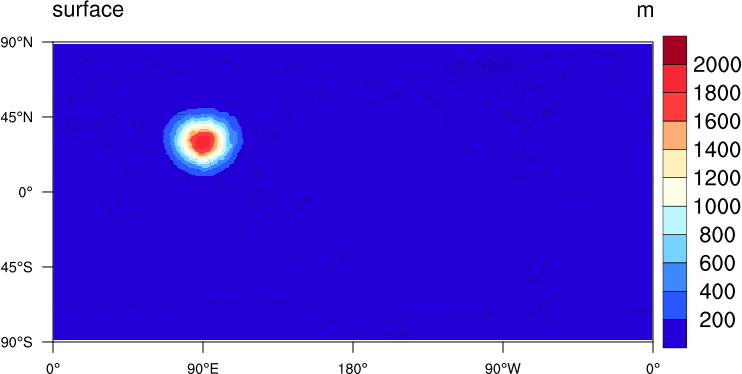
\includegraphics[width=0.95\linewidth]{pictures/surface-small.png}
\caption{Topography of the test case}\label{fig:mountain}
\end{figure}

The v-component of the wind speed is is initialized with zero at all grid points, the initial conditions for the u-component are shown in Fig. \ref{fig:u-initial}.

\begin{figure}[h!]%
\centering
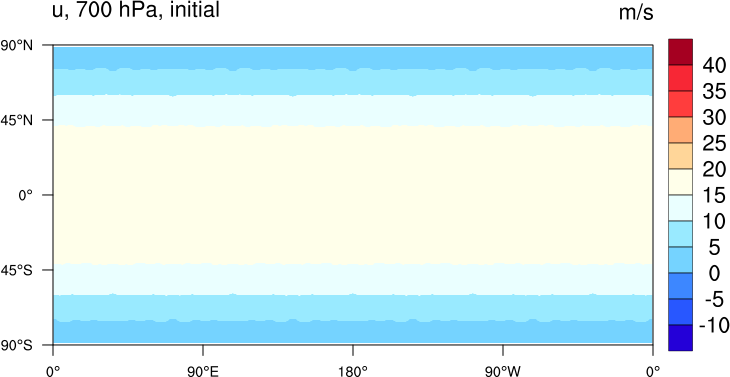
\includegraphics[width=0.95\linewidth]{pictures/u_initial_v2-small.png}
\caption{Spatial distribution of the initialized u-component at 700 hPa}\label{fig:u-initial}
\end{figure}



\subsubsection{Results after 16 days}



The u-component after sixteen days of simulation at 700 hPa is shown in Fig. \ref{fig:u-16}, the corresponding v-component is shown in Fig. \ref{fig:v-16}, and Fig. \ref{fig:vorticity-16} shows the vorticiy.

\begin{figure}[h!]%
\centering
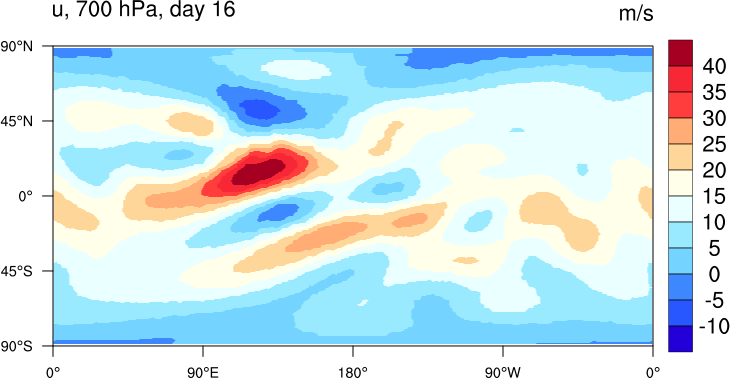
\includegraphics[width=0.95\linewidth]{pictures/u-day-16-small.png}
\caption{Spatial distribution of u-component after 16 days of simulation at 700 hPa}\label{fig:u-16}
\end{figure}


\begin{figure}[h!]%
\centering
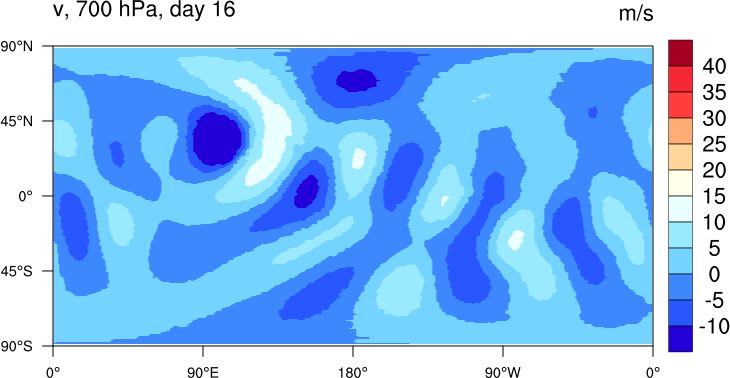
\includegraphics[width=0.95\linewidth]{pictures/v_day_16-small.png}
\caption{Spatial distribution of v-component after 16 days of simulation at 700 hPa}\label{fig:v-16}
\end{figure}


\begin{figure}[h!]%
\centering
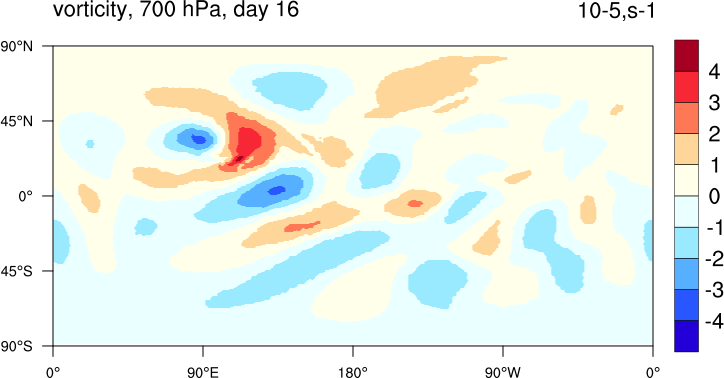
\includegraphics[width=0.95\linewidth]{pictures/vorticity_16-o.png}
\caption{Spatial distribution of the vorticity after 16 days of simulation at 700 hPa}\label{fig:vorticity-16}
\end{figure}





\subsubsection{Input Data}

With the exception of the grid file no further input files are necessary. 




\section{Running the Model (Real Case)}
\label{chap:UG_running_model}


The ICON code, as checkout from the SVN repository, does not include runscripts. Instead the run directory (\verb+$ICONDIR/run/+) includes several descriptor files for building grids, defining experiments and post-processings. There exist three different types of descriptor files with prefixes \verb+grid, exp, post+:

\begin{itemize}
 \item \verb+grid.<name>+: to configure the grid generator, see chapter \ref{chap:UG_grid_generation} for more details. It is recommended to use pre-built grids. For details, see section \ref{chap:prebuilt_grid}.
 \item \verb+exp.<name>+: to define the namelist, which determinate the experiments.
 \item \verb+post.<name>+: to define post-processing.
\end{itemize}

\subsection{Input Data}

Generally ICON requires the following input data: Grid files, external parameters, initialization (DWD analysis or IFS), input fields for radiation.

\subsubsection{Grid Files}\label{sec:grid_input}

In order to run ICON, it is necessary to have the horizontal grid information as an input parameter. This information is stored within so-called grid files. For a ICON run, one global grid file is necessary. Additionally, if you want to nest, grid files of the nested domains are necessary, too. To improve the performance of ICON, a (optional) reduced radiation grid for each domain may be used. 

The naming of the ICON-Grid is as follows: The initial icosahedron grid is refined by \textless n\textgreater -secting the edges, and further refinement is obtained by iteratively bisecting the created edges. The grid produced at the \textless k\textgreater refining iteration is named "R\textless n\textgreater B\textless k\textgreater". For further details, see the ICON Technical Documentation.

It is recommended to use pre-built grids. Further information can be found in chapter \ref{chap:prebuilt_grid}. For building own grids, the reader is referred to chapter \ref{chap:UG_grid_generation}. The names of the grid files have to be specified within the \verb+grid_nml+:

\begin{verbatim}
&grid_nml
dynamics_grid_filename = "<INSERTFILENAME>"
radiation_grid_filename = "<INSERTFILENAME>"
\end{verbatim}

\subsubsection{External Parameters}\label{InputReal:Ext}

ICON requires geographical localized datasets like the topographic height of the earth surface, the plant cover, the distribution of land and sea and, dependent on the schemes used, a variety of other so called external parameters. The EXTPAR software system (EXTPAR - External Parameter for Numerical Weather Prediction and Climate Application) is able to generate external parameters for the different models GME, COSMO, HRM and ICON. The software can run on a UNIX or Linux systems where the raw data is stored. It allows operators (experienced users) running the scripts to create new external parameters controlled by user specifications like the model domain. For a more detailed overview of EXTPAR, the reader is referred to the User and Implementation Guide of EXTPAR. 

The name of the EXTPAR file which has to be read by ICON can be specified as follows:

\begin{verbatim}
&extpar_nml
extpar_filename = "<INSERTFILENAME>"
\end{verbatim}

If not specified explicitly, ICON uses the following file name: \newline
\verb+"<path>extpar_<gridfile>"+.\newline
 \verb+<path>+ and \verb+<gridfile>+ are then replaced at runtime by ICON.

\subsubsection{Initialization}\label{InputReal:Ini}

For the initialization of ICON, input data from either DWD or IFS is needed. 

In case of DWD (init\_mode=1) a first guess and an analysis is required: 
\begin{verbatim}
&initicon_nml
dwdfg_filename = "<INSERTFILENAME>"
dwdana_filename = "<INSERTFILENAME>"
\end{verbatim}

If not specified explicitly, ICON uses the following file names: \newline 
\verb+"<path>dwdFG_R<n>B<k>_DOM<idom>.nc"+ and \newline
\verb+"<path>dwdana_R<n>B<k>_DOM<idom>.nc"+. \newline
\verb+<path>+, \verb+<n>+, \verb+<k>+ and \verb+<idom>+ are then replaced at runtime by ICON according to the chosen gridfile (see \ref{sec:grid_input}). The variable \verb+<idom>+ is an index for the domain on which the calculations are performed. \verb+<idom>=0000+ is reserved for a reduced radiation grid, \verb+<idom>=0001+ for the global domain, higher numbers are used for nested domains. NETCDF as well as GRIB2 input can be used.

In case of IFS (init\_mode=2) an analysis is required. It has to be in \netcdf: 
\begin{verbatim}
&initicon_nml
ifs2icon_filename = "<INSERTFILENAME>"
\end{verbatim}

If not specified explicitly, ICON uses the following file name: \newline 
\verb+"<path>ifs2icon_R<n>B<k>_DOM<idom>.nc"+. \newline
\verb+<path>+, \verb+<n>+, \verb+<k>+ and \verb+<idom>+ are then replaced at runtime by ICON according to the chosen gridfile (see \ref{sec:grid_input}). The variable \verb+<idom>+ is an index for the domain on which the calculations are performed. \verb+<idom>=0000+ is reserved for a reduced radiation grid, \verb+<idom>=0001+ for the global domain, higher numbers are used for nested domains.

\subsubsection{Radiation}\label{InputReal:Rad}

ICON requires input fields for the RRTM radiation scheme. The file names are specified as follows:

\begin{verbatim}
&nwp_phy_nml
lrtm_filename = "<INSERTFILENAME>" 
cldopt_filename = "<INSERTFILENAME>"
\end{verbatim}

If not specified explicitly, ICON uses the following file names: \newline 
\verb+"rrtmg_lw.nc"+ and \newline
\verb+"ECHAM6_CldOptProps.nc"+.

The files can be found within \verb+$ICONDIR/data+.

\subsection{Creating a Runscript}

To create a runscript, new users are advised to use the namelist descriptor file \verb+exp.nh-oper+ which contains recently recommended namelist settings. It might be necessary to account for the file names and paths of the input data. Additionally, machine dependent settings need to be added to this script to obtain a runscript. For some architectures, this step can be performed by using the make runscript environment as shown in \ref{sec:make_runscript}. In the following, example settings for DWD CRAY are listed.

\begin{Verbatim}[frame=single]
CRAY EXAMPLE: Environment variables
#!/bin/ksh
#==============================================================
#PBS -q xc_normal
#PBS -l select=?:ncpus=?:mpiprocs=?:ompthreads=?:mem=?gb
#PBS -l place=scatter
#PBS -j oe
#PBS -N <<Jobname>>

export MPICH_RMA_OVER_DMAPP=1
\end{Verbatim}

\begin{Verbatim}[frame=single]
CRAY EXAMPLE: Namelists
<<Place your namelists e.g. from exp.nh_oper here>>
\end{Verbatim}

\begin{Verbatim}[frame=single]
CRAY EXAMPLE: Submitting a job
aprun                                    \
  -n <<INSERT: Total number of MPI Tasks>>            \
  -N <<INSERT: MPI Tasks/Node>>       \
  <<INSERT: Hyperthreading e.g. 2 -> 20 physical -> 40 "virtual" cores>> \
  -d <<INSERT: Threads/MPI Task>>     \
  -m <<INSERT: Amount of memory to use>> control_model
\end{Verbatim}


\subsection{Restart}

A restart of the model requires a restart file that has to be created by a 
previous model run. In the following the procedures and the corresponding namelist settings are explained.

\subsubsection{Creating the initial restart file:}

The first job in a series of model runs creates the first restart file.
To do so we have to use the following namelist switches.

\begin{verbatim}
&master_nml
lrestart = .FALSE. 
\end{verbatim}

In addition we have to prescribe at which time interval the job should produce a restart file:

\begin{verbatim}
&io_nml
dt_checkpoint = "<Insert time in seconds>" 
\end{verbatim}


The ICON run then creates restart files for each domain 1, ..., \verb+n_dom+, and for each restart
output time step. 

The filenames are generic and look like:

\begin{verbatim}
 "<gridfile>_restart_<modeltype>_<timestamp>.nc", 
\end{verbatim}

An example would be:

\begin{verbatim}
 "iconR2B06_DOM01_restart_atm_20110101T001200Z.nc"    (NetCDF format)
\end{verbatim}
   
This filename can be customized using the namelist parameter:
    
     
\begin{verbatim}
&mo_run_nml
restart_filename = "<INSERTFILENAME>" 
\end{verbatim}

This file contains:

\begin{itemize}
\item{data} 
\item{namelists}
\item{several attributes}
\end{itemize}


Note:
    -  ICON reads the namelists only once and assumes that these
       are identical for all domains.
    -  Since we do not know about the total number of domains at startup,
       we have to ask the current restart file for the attribute \verb+"n_dom"+.


For each domain 1, ..., \verb+n_dom+, a symbolic link is generated with the generic name: 

 \verb+"restart_<modeltype>_DOMxx.nc"+

     
     
 
Note:
    -  The domain-dependent suffix "...DOMxx" is also required for 
non-nested setups.

    


\subsubsection{Running the model in the restart mode:}

ICON has to be informed that you want to carry out a restart run:

\begin{verbatim}
&master_nml
lrestart = .TRUE. 
\end{verbatim}

The generic link \verb+"restart_<modeltype>_DOMxx.nc"+ is used by the restart run to point to the last written restart file of the previous model run. 


\subsubsection*{Chain of restart runs}

If a chain of restart runs is foreseen it is recommended to use the namelist parameter
\verb+dt_restart+. 

\begin{verbatim}
&time_nml
dt_restart = "<Insert time in seconds>" 
\end{verbatim}


In this case only one restart file is produced by each model run and after writing the restart file the job stops.

Note:- \verb+dt_restart+ and \verb+dt_checkpoint+ have to be selected carefully. 
 


\subsubsection*{Asynchronous restart:} 

The restart can be handled by separated processors. The number of restart processors can be chosen by the user. The corresponding namelist parameter is:

\begin{verbatim}
&parallel_nml
num_restart_procs = n
\end{verbatim} 

n is the number of processors used for restart.


\subsection{Make Runscript Environment}\label{sec:make_runscript}


A full listing of descriptor files you will find in \verb+$ICON/run/+. 

After configuration and compiling (chapter \ref{chap:UG_config_compil}) these descriptor files can be transformed into runscripts, which should include the necessary system dependent parameters and the execution section \verb+exec.icon+ (\verb+$ICONDIR/run/exec.iconrun+), which starts the actual integration. This transformation is done in \verb+$ICONDIR+ by:

\begin{small}
 \begin{verbatim}
  ./make_runscripts
 \end{verbatim}
\end{small}

This transforms every existing descriptor file in \verb+$ICONDIR/run/<type>.<name>+ into a ready-to-use run script \verb+$ICONDIR/run/<type>.<name>.run+

For illustration there exists also 

\begin{small}
 \begin{verbatim}
  ./make_my_runscripts
 \end{verbatim}
\end{small}

which transforms a single descriptor file into a run script. This file is an exemplary file and you can see how to define run parameters.

An exemplary descriptor file for a operational run is \verb+exp.nh_oper+.

\textbf{Note:} if you change, or create a descriptor you will need to (re)create the run script in order for the changes to take effect.

To run a script \verb+<type>.<name>.run+, either for creating grids or making an experiment or doing post-processing, go to the \verb+./run+ folder

\begin{small}
  \begin{verbatim}
   cd run
  \end{verbatim}
\end{small}

and use the job submission command, which depends on your machine:

\begin{small}
  \begin{verbatim}
   [<submit>] <type>.<name>.run
  \end{verbatim}
\end{small} 

\verb+[<submit>]+ is something like: \verb+{llsubmit,qsub}+

\textbf{Note:} \underline{Before} (!) running an experiment, the ICON grids must be available to the model. For this purpose, either pre-built grids and ExtPar Data can be used (see Sec. \ref{chap:prebuilt_grid}) or create own grids (\ref{chap:UG_grid_generation}). For a new user, it is suggested to use pre-built grids first.

\section{Pre-built Grids and ExtPar Data}\label{chap:prebuilt_grid}
A list of grid files has been pre-built for the ICON model together with the corresponding reduced radiation grids and the external parameters.

\begin{enumerate}

\item The \textbf{primary storage} location for ICON grids is
\begin{small}
 \begin{verbatim}
  blizzard:/pool/data/ICON/grids/public 
 \end{verbatim}
\end{small}
\item Every 24h the contents of the primary storage directory are mirrored to DWD's HPC.
\item Every 24h the contents of the primary storage directory are mirrored to a public web site:
\href{http://icon-downloads.zmaw.de}{http://icon-downloads.zmaw.de}.
\end{enumerate}

Each grid file consists of a NetCDF file and a GPG signature file\\ 
(\href{http://de.wikipedia.org/wiki/GNU\_Privacy\_Guard}{http://de.wikipedia.org/wiki/GNU\_Privacy\_Guard}).\\ 
The signature file makes sure that a grid file is complete and verifies the authorship.

\subsection{Grid file nomenclature}
The grids are identified by
\begin{itemize}
\item a \textbf{centre} number
\item a \textbf{subcentre} number
\item a \textbf{numberOfGridUsed}\\
which is simply an integer number, increased by one with every new \lq official\rq\ grid.  
\end{itemize}

The grid files and the external parameter files are named accordingly, e.g.,
\begin{small}
 \begin{verbatim}
  icon_grid_0001_RxxByy_G.nc
  icon_extpar_0001_RxxByy_G.nc 
 \end{verbatim}
\end{small}
where the name components are as follows:
\begin{small}
 \begin{verbatim}
 icon _	grid   _ 0001 _	R 02 B 06 _	R                   .nc 
                                     (radiation/reduced)
 icon _ extpar _ 0002 _	  03   07 _	G                   .nc
                                     (global)         
 \end{verbatim}
\end{small}

The \verb+numberOfGridUsed+ parameter is part of the file name (0001, ...) and makes this file name unique.

In general, a lookup table is required to find the actual file name to which a set of these parameters corresponds. 
This \lq table file\rq\ is located under 
\begin{center}
  {\tt http://icon-downloads.zmaw.de/dwd\_grids.xml} 
\end{center}
(the table file itself is under version control: \href{https://svn.zmaw.de/svn/icon\_grid\_table}{https://svn.zmaw.de/svn/icon\_grid\_table}). 



%\subsection{How does the XML grid description look like?}
%The table is stored in XML format, which is more or less human-readable. It consists of paragraphs of the following form:
%
%\begin{small}
% \begin{verbatim}
%    <grid  oper                = "yes"
%           number_of_grid_used = "2"
%           centre              = "78"
%           subcentre           = "255"
%           type                = "horizontal">
%     <description>
%           Global R02B06 grid.
%           40 km resolution
%     </description>
%     <uri>grids/public/edzw/icon_grid_0002_R02B06_G.nc</uri>
%     <extpar>
%      <uri>grids/public/edzw/icon_extpar_0002_R02B06_G.nc</uri>
%      <description>Globcover-based data set.</description>
%     </extpar>
%    </grid>
% \end{verbatim}
%\end{small}
%
%\begin{itemize}
%\item The optional oper attribute allows to mark a specific grid as operational. 
%\item The \verb+<description>+ tag allows to describe the grid properties in a few words. 
%\end{itemize}
%
%The XML file can also be \textbf{viewed in a web browser}
%\begin{small}
% \begin{verbatim}
%  firefox --no-remote ${ICON_XML_GRID_TABLE}
% \end{verbatim}
%\end{small}
%
%where the table layout is then defined by the XSL definitions in \verb+xml/dwd_grids.xsl+. 
%\begin{itemize}
%\item The XML file will later be available in tabular form on the public grid web site. 
%\end{itemize}
%
%Finally, the XML file contains information on \textbf{associated grids} (e.g., refinement hierarchies):
%\begin{small}
% \begin{verbatim}
%    <gridset>
%      <description>
%        Global R02B04 grid hierarchy without nests.
%      </description>
%      <grid number_of_grid_used = "9"  
%            centre              = "78"
%            subcentre           = "255"
%            type                = "horizontal" />
%      <grid number_of_grid_used = "10"  
%            centre              = "78"
%            subcentre           = "255"
%            type                = "horizontal" />
%    </gridset>
% \end{verbatim}
%\end{small}

\section{Grid Generation}
\label{chap:UG_grid_generation}

\subsection{ICON atmosphere grids}

The ICON horizontal spherical grid is based on the projection of the icosahedron on the sphere. This is a 2-dimensional grid, representing the earth's surface. The ICON grids need to be created, stored as \netcdf~ files, and consequently used by the ICON model. Alternatively, already stored grids may be used.

The initial icosahedron grid is refined by \textless n\textgreater -secting the edges, and further refinement is obtained by iteratively bisecting the created edges. The grid produced at the \textless k\textgreater refining iteration is named "R\textless n\textgreater B\textless k\textgreater", and the corresponding \netcdf -file is \verb+"iconR<n>B<k>-grid.nc"+. The grid files, after their creation, are located in the \verb+./grids+ folder. For more detailed information about horizontal ICON grids the reader is referred to the ICON technical documentation.

Examples of grids are in \verb+./grids+. More information can be found in: \\ 
\verb+$ICONDIR/doc/technical/icon_grid.pdf+.


The example given below shows the namelist parameters for generating a global R2B6 grid.

\begin{Verbatim}[frame=single]
EXAMPLE Grid Generation of a R2B6 grid
#!/bin/ksh
#--------------------------------------
# Creation of atmosphere grids for ICON
#----------------------------------------
# ICON grid generator namelist parameters
#
# For a complete list see Namelist_overview and Namelist_overview.pdf
#
# nroot       =  Number of sections into which the edges of the original 
#                icosahedron are divided in the initial refinement step.
#                (icosahedron = "grid -1" --> "nroot" grid = grid "0")
#                
# grid_levels =  Number of refinement steps applying edge bisection,
#                follows the initial "nroot" refinement step.
#                (grid "0" --> grid "1" --> ... --> grid "grid_levels")
#
# itype_optimize grid optimization method applied from grid level 1 onward.
#                i | optimization    | suffix fo grid output file
#                ------------------------------------------------
#                0 | none            | noo
#                1 | Heikes Randall  | hro
#                4 | spring dynamics | spr
#
# beta_spring = Tuning parameter for spring dynamics to be chosen in the 
#               range [0.9,1.1]. Weights the target length between the
#               grid points.
#
#----------------------
# First generate graphs
R=2    # nroot (the first dissection will be a bisection)
B=6    # highest grid level to reach (number of consequent bisections)
maxlev_optim=6  # highest grid level to apply optimizations

cat > NAMELIST_GRAPH << EOF
&graph_ini 
  nroot       = ${R}
  grid_levels = ${B}
/
EOF

echo global_graph_generator null > $commandFile
${start} ${run_commmand}
check_error $? "global_graph_generator"

#------------------------------------------------------
# Generate grids using the spring dynamics optimization
cat > NAMELIST_GRID << EOF
&grid_ini
  nroot       = ${R}
  grid_levels = ${B}
/
&grid_options
  itype_optimize = 4     ! 1 = Heikes-Randall, 4 = spring dynamics
  maxlev_optim = $maxlev_optim       ! the maximum level to optimize
/
EOF
\end{Verbatim}

ICON gives the possibility to nest subdomain within a parent grid. The example below gives the namelist parameters for generating a nested grid (patch). The root bisection of the patch in this example starts with the fourth level of the bisections of the global model.

\begin{Verbatim}[frame=single]
EXAMPLE Nested grid based on the global grid described before. 
#----------------------------------
# Next the patches will be created.
# If the pathes are not needed then uncomment the next exit command
#
#exit
#-------------------------------
#
# ICON prepare_gridref namelist
#
# Parameter overview:
#
# grid_root: Number of root bisections
#
# start_lev: Grid level of global domain
#
# n_dom:     Total number of model domains (including the global one)
#
# parent_id: List of parent domain ID's (starts at first nested domain,
#            which has ID=2)
#
# l_circ:    true = circular subdomains, false = 
#            rectangular (lat/lon) subdomains
#
# l_rotate:  true: rotate center point into equator in case of l_circ=false
#            this yields truly rectangular subdomains, whereas subdomains
#            are conical otherwise because of the convergence of meridians
#
# NOTE:      For subdomains crossing a pole, either l_circ=true 
#            or l_rotate=true is required
#
# l_plot:    true: Generates GMT files for domain configuration
#
# NOTE:      The following parameters have to be specified for each nested
#            domain!
#
# radius:    radius (deg) of nested domains  (for l_circ=true)
#
# center_lon: Center longitude of nested domains
#
# center_lon: Center latitude of nested domains
#
# hwidth_lon: half-width longitude of nested domains (for l_circ=false)
#
# hwidth_lat: half-width latitude of nested domains (for l_circ=false)
#
#-------------------------------------------------------
# suffix of grid files which specifies optimization type
# (without optimization leave empty)
#OPTFIX=spr0.90_M4
# NOTE: _M4 means that maxlev_optim = 4 has to be set in the grid generator
# maxlev_optim is not needed for Heikes-Randall optimization
#
#-------------------------------------
# Create plots of domain configuration
PLOTS=.false.
#
cat > NAMELIST_GRIDREF << EOF
&gridref_ini 
  grid_root  = 2
  start_lev  = 4
  n_dom      = 2
  parent_id  = 1,
  l_circ     = .true.
  l_rotate   = .true.
  l_plot     = .true.
  radius     =  30.,
  center_lon =  -90.,
  center_lat =  40.,
  hwidth_lon =  55.,
  hwidth_lat =  55.,
  bdy_indexing_depth = 14
/
EOF
\end{Verbatim}



\subsection{Information contained in grid files}

The ICON grids are treated as a general unstructured grid, so the grid \netcdf -files contain the full information of the location and the connectivity of all the grid entities (cells, edges and vertices). The grid nesting hierarchy information is also included.

Some basic variables that may be useful for plotting are:

\begin{small}
  \begin{verbatim}
double clon(cell)                : longitude of cell centers [radian]
double clat(cell)                : latitude  of cell centers [radian]
double clon_vertices(cell, nv)   : longitudes of the vertices of the cell [radian]
double clat_vertices(cell, nv)   : latitudess of the vertices of the cell [radian]
double elon(edge)                : longitude of edge midpoint [radian]
double elat(edge)                : latitude  of edge midpoint [radian]
double elon_vertices(edge, no)   : longitudes of the vertices of the edges [radian]
double elat_vertices(edge, no)   : latitudes  of the vertices of the edges [radian]
double vlon(vertex)              : longitude of vertices [radian]
double vlat(vertex)              : latitude  of vertices [radian]
...
double cell_area(cell)           : area of grid cell [m2]
double cell_elevation(cell)      : elevation at the cell centers [m]
int    cell_sea_land_mask(cell): sea (-2 inner, -1 boundary) 
                                   land (2 inner, 1 boundary) mask for the cell
...
double edge_length(edge)         : lengths of edges of triangular cells [m]
double dual_edge_length(edge)   : lengths of dual edges (distances between
                                   triangular cell circumcenters) [m]
...
  \end{verbatim}
\end{small}

For a full listing of variables contained in a grid file, for instance in iconR2B04-grid.nc, use:

\begin{small}
  \begin{verbatim}
   ncdump -h iconR2B04-grid.nc  
  \end{verbatim}
\end{small}

or

\begin{small}
  \begin{verbatim}
   cdo sinfov iconR2B04-grid.nc
  \end{verbatim}
\end{small}

\subsection{Viewing/plotting grids}

In order to plot an icon grid you should ensure that \verb+ncl-6.0+ and \verb+cdo-1.5.4+ is available on your machine. Then go to the \verb+$ICONDIR/grids/+ folder and give:

\begin{small}
  \begin{verbatim}
alias iplot="ncl $ICONDIR/scripts/postprocessing/tools/icon_plot.ncl 
'altLibDir="$ICONDIR/scripts/postprocessing/tools/"'" iplot 'iFile="<grid file name>"' 
'mapType="ortho"' 'varName="cell_sea_land_mask"' 'oType="png"' 'showGrid=True' 
'lStrg="Cell sea land mask"' 'bStrg=""'
  \end{verbatim}
\end{small}



The above example will plot cell sea land mask. More details on plotting can be found at the Visualization chapter.

The \verb+$ICONDIR/run/post.plot_icon_grids+ script can be used to plot nested grids. Go to \verb+$ICONDIR/run/+ folder and give:

\begin{small}
  \begin{verbatim}
   ./post.plot_icon_grids  
  \end{verbatim}
\end{small}

A PDF-file with a plot of the iconR2B04\_DOM01 and iconR2B05\_DOM02 grids will appear on your screen. (Note that this process is time consuming.)

\newpage
\subsection*{Discussion}
%This section is for discussion only. Please add your notes, your name and date.
Document last edited by \textit{B Vogel} on \textit{27-06-2014}.
